% Generated by eval/realworld/scripts/05-charts.py from eval/realworld/results. Do not edit.
\subsection{Local open-weight runs and other record systems}
\label{sec:realworld}

The artificial evaluation mocks the provider. This subsection does not. Ollama 0.40.7 served \texttt{llama3.2:3b} (Llama 3.2, 3.2B, Q4\_K\_M, digest \texttt{a80c4f17acd5}, 2.0~GB) on the same host as the other measurements (Node v24.22.1, 4~vCPU, 15.63~GB RAM, no GPU). Lattice called it through the OpenAI-compatible adapter with no API key. The adapter does not send temperature or a token cap; a fetch wrapper added both, and that fact is part of the record. No vision model was loaded. No hosted provider key was present.

On the one-line prompt ``Reply with the single word pong,'' temperature 0, five paired trials, the median plain HTTP call was 278~ms. A signed Lattice run of the same task was 559~ms and an unsigned Lattice run was 745~ms (Figure~\ref{fig:rw-latency}). The first plain call, 4845~ms, is a cold start and pulls the mean up; the median does not. The signed median is lower than the unsigned median. That gap is generation noise, not a claim that signing is faster. What is stable is the time spent outside the provider HTTP call: 0.439\% of end-to-end latency at the signed median (minimum 0.335\%, maximum 2.469\%). The Lattice prompt body was 382 characters against a one-line plain prompt, so most of the extra wall time is a larger prefill, not the signature. The short signed receipt was 996~bytes.

A refund-policy question with a \texttt{mustCite} invariant passed on all three temperature-0 runs and all three temperature-0.7 runs. Each temperature produced one identical answer across its three trials (n=3). The two temperatures did not produce the same sentence. All 6 signed receipts verified, replayed offline, matched the output hash, and a one-character edit was detected (6/6). A synthetic support ticket containing an email, a US phone number, and a dashed SSN was flagged by those three detectors. The model's answer contained none of them, the \texttt{noPII} invariant passed, and the signed receipt did not contain the planted strings. A two-step agent called \texttt{lookup\_policy} once and answered; the returned agent object carried no receipt. A two-agent crew completed in 3 iterations with 4 receipts.

On the public sets the same detectors are weaker than on the synthetic harness, and the gap is the result (Figure~\ref{fig:rw-pii}). ai4privacy/pii-masking-300k English validation (revision \texttt{c8c77895a005}, 7,946 documents; academic, non-commercial, no redistribution) gives email precision 0.955 and recall 0.979 (1533 documents with a gold email). US SSN precision is 0.325 and recall 0.436. US phone precision is 0.316 and recall 0.333. Of the SSN false positives, 1,074 overlap a passport span: a 9-digit passport is the same shape as an SSN, and the detector cannot tell them apart. Of the phone false positives, 629 overlap a social-security span. There is no gold credit-card span in this file; the card detector fired on 7 documents anyway. Among 1,070 US-shaped SSN spans, the single match the API returns overlaps 663. It misses 370 because that one match fell on a different number earlier in the document, and 37 because it matched nothing. Gretel English finance test (Apache-2.0, revision \texttt{7b844d167385}, 2,891 rows) is the same pattern at smaller n: email recall 0.934, SSN precision 0.161. ASQA dev (Apache-2.0, revision \texttt{084060f16b46}, 948 answers) is a loss for \texttt{mustCite}. A gold Wikipedia title occurs as a substring in 525 answers, but the invariant accepts at least one gold title in 7. Only 2 answers use a square-bracket citation. The check is syntactic. It does not score whether a citation supports the claim.

Table~\ref{tab:rw-matrix} wraps the same recorded request and response bytes. Lattice's receipt and Sello's encrypted receipt (mock transparency log, not the public log) omit the planted strings. An AFR log with disclosure encryption also omits them; the default AFR log contains them. Janus's local evidence appender stores the payload in the clear and the byte edit fails \texttt{verify.SegmentDir}. A sealed NovaFabric capsule (self-asserted ECDSA key, no RFC~3161 timestamp) fails \texttt{nova verify} after a newline is appended to stdout, and the capsule contains the planted text. \texttt{nova validate} on that edited capsule still exits 0. cosign \texttt{sign-blob} with a local key, not Fulcio or Rekor, detects a byte edit and signs the plaintext log. in-toto's DSSE link detects a byte edit and does not embed the plaintext. A hash chain detects an edit that leaves the stored hashes untouched and accepts a rebuilt chain, because nothing outside the file anchors the head. NovaFabric's HMAC record has the same shape with a shared secret: an edit fails, and a re-sign with that secret passes. OpenTelemetry GenAI spans and a plain JSON log have no integrity check; both store the transcript. TrustTrack has no implementation we could run. Langfuse was not started: this host has no Docker daemon. Figure~\ref{fig:rw-bytes} is the byte column.

\begin{figure}[t]
\centering
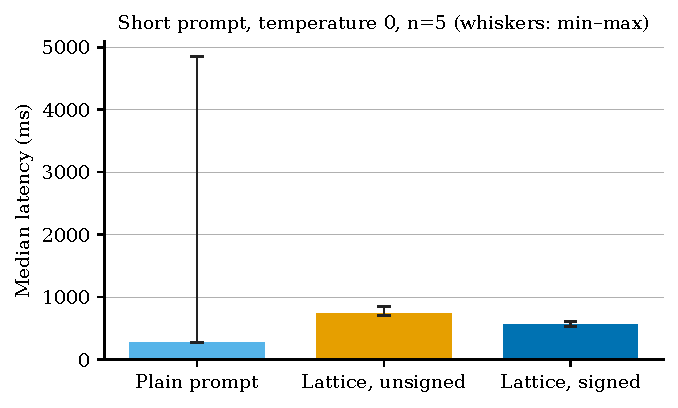
\includegraphics[width=\linewidth]{rw-latency.pdf}
\caption{Median latency of a one-line completion. Whiskers run from the minimum to the maximum of five trials. The plain arm sends only that line. The Lattice arms send the adapter's packed prompt.}
\label{fig:rw-latency}
\end{figure}

\begin{figure}[t]
\centering
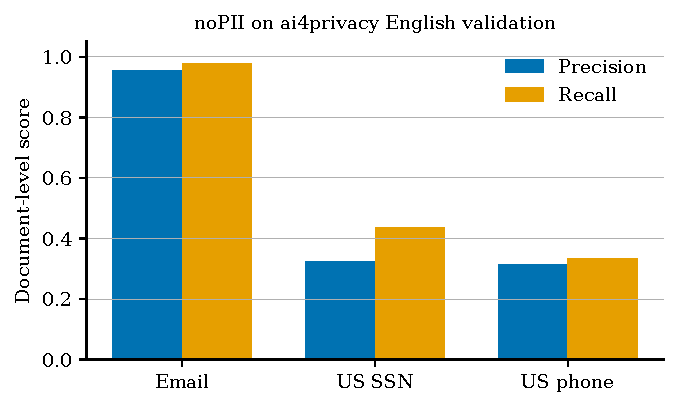
\includegraphics[width=\linewidth]{rw-pii.pdf}
\caption{Document-level precision and recall of the default \texttt{noPII} detectors on ai4privacy English validation. US SSN and US phone lose to identifier types that share their shape.}
\label{fig:rw-pii}
\end{figure}

\begin{figure}[t]
\centering
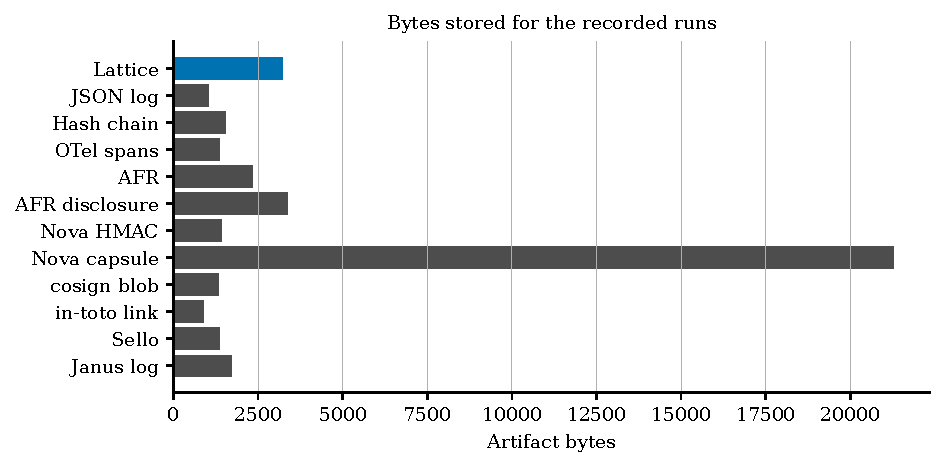
\includegraphics[width=0.92\linewidth]{rw-bytes.pdf}
\caption{Bytes retained for the recorded runs. The NovaFabric bar is one sealed capsule, not three hash receipts. AFR disclosure is the encrypted archive.}
\label{fig:rw-bytes}
\end{figure}

\input{realworld-matrix.tex}
